\documentclass{apcalc}
\title{Unit 9: Parametric Equations, Polar Coordinates, and Vector-Valued Functions}
\author{Paul Wang}
\date{November 2026}
\volume{Study Guide 9 of 10 (topics 9.1--9.9)}
\shorttitle{Unit 9 --- Study Guide}
\begin{document}
\maketitle

\begin{abstract}
Unit 9 is BC-only and carries 10--15\% of the multiple-choice section. It reuses derivatives and integrals on curves that are not graphs of functions: parametric curves, particles moving in the plane, and polar curves. Every year one free-response question is either a particle moving in the plane (velocity vector, speed, position, distance) or a polar region (area, $\frac{dr}{d\theta}$, $\frac{dy}{dx}$), and the calculator part often carries it. This guide states the unit in ten rules (R9.1--R9.10) across five sections. The \emph{Unit 9 Practice Set} uses the same section numbers.
\end{abstract}
\keywords{parametric equations, $\frac{dy}{dx}$ and $\frac{d^2y}{dx^2}$ for parametric curves, arc length, vector-valued function, velocity vector, speed, polar coordinates, polar area.}

\section*{Router}
\begin{router}
$x(t)$, $y(t)$: slope of the curve & $\frac{dy}{dx}=\frac{y'(t)}{x'(t)}$ & R9.1 \\
second derivative of a parametric curve & $\frac{d}{dt}\left(\frac{dy}{dx}\right)\Big/\frac{dx}{dt}$ & R9.2 \\
length of a parametric path & $\int\sqrt{x'(t)^2+y'(t)^2}\,dt$ & R9.3 \\
speed of a particle & $\sqrt{x'(t)^2+y'(t)^2}$ & R9.4 \\
position from a velocity vector & $x(b)=x(a)+\int_a^bx'(t)\,dt$, same for $y$ & R9.5 \\
polar to rectangular & $x=r\cos\theta$, $y=r\sin\theta$ & R9.6 \\
slope of a polar curve & $\frac{dy}{dx}=\frac{dy/d\theta}{dx/d\theta}$ with $y=r\sin\theta$, $x=r\cos\theta$ & R9.7 \\
``is the point moving toward the origin?'' & sign of $\frac{dr}{d\theta}$ together with the sign of $r$ & R9.8 \\
area inside a polar curve & $\frac12\int_\alpha^\beta r^2\,d\theta$ & R9.9 \\
area between two polar curves & $\frac12\int(r_{\text{out}}^2-r_{\text{in}}^2)\,d\theta$ & R9.10 \\
\end{router}

\section{Parametric curves and their derivatives (9.1--9.2)}

\begin{rulebox}{R9.1}{First derivative of a parametric curve}
For $x=x(t)$, $y=y(t)$: $\dfrac{dy}{dx}=\dfrac{dy/dt}{dx/dt}$ when $\frac{dx}{dt}\neq0$. Horizontal tangent: $\frac{dy}{dt}=0$, $\frac{dx}{dt}\neq0$. Vertical tangent: $\frac{dx}{dt}=0$, $\frac{dy}{dt}\neq0$.
\end{rulebox}

\begin{rulebox}{R9.2}{Second derivative}
$\dfrac{d^2y}{dx^2}=\dfrac{\frac{d}{dt}\left(\frac{dy}{dx}\right)}{dx/dt}$. Differentiate the slope with respect to $t$, then divide by $\frac{dx}{dt}$ again. It is \emph{not} $\frac{y''(t)}{x''(t)}$.
\end{rulebox}

\begin{example}{tangent line and concavity}
$x=t^2$, $y=t^3-3t$. $\frac{dy}{dx}=\frac{3t^2-3}{2t}$. At $t=2$: point $(4,2)$, slope $\frac94$. $\frac{d}{dt}\frac{dy}{dx}=\frac{d}{dt}\left(\frac32t-\frac{3}{2t}\right)=\frac32+\frac{3}{2t^2}$, so $\frac{d^2y}{dx^2}=\frac{\frac32+\frac{3}{2t^2}}{2t}$; at $t=2$: $\frac{15/8}{4}=\frac{15}{32}>0$, concave up. \answer{$y=2+\frac94(x-4)$; concave up.}
\end{example}

\section{Parametric arc length (9.3)}

\begin{rulebox}{R9.3}{Arc length of a parametric curve}
$L=\displaystyle\int_a^b\sqrt{\left(\frac{dx}{dt}\right)^2+\left(\frac{dy}{dt}\right)^2}\,dt$, the integral of speed. If the curve retraces itself, this counts the retraced part again (it is distance traveled).
\end{rulebox}

\begin{example}{a circle}
$x=3\cos t$, $y=3\sin t$, $0\le t\le\pi$: speed $\sqrt{9\sin^2t+9\cos^2t}=3$, so $L=3\pi$, half the circumference.
\end{example}

\section{Vector-valued functions and planar motion (9.4--9.6)}

\begin{rulebox}{R9.4}{Velocity, acceleration, speed}
Position $\langle x(t),y(t)\rangle$; velocity $\langle x'(t),y'(t)\rangle$; acceleration $\langle x''(t),y''(t)\rangle$. Speed $=\sqrt{x'(t)^2+y'(t)^2}$ (a number, not a vector). The particle moves left when $x'<0$, up when $y'>0$. At rest: both components 0.
\end{rulebox}

\begin{rulebox}{R9.5}{Position and distance from velocity}
$x(b)=x(a)+\int_a^bx'(t)\,dt$ and $y(b)=y(a)+\int_a^by'(t)\,dt$. Total distance traveled $=\int_a^b\sqrt{x'(t)^2+y'(t)^2}\,dt$. Displacement is the vector $\langle\int x',\int y'\rangle$.
\end{rulebox}

\begin{example}{a particle in the plane (calculator)}
$v(t)=\langle e^{\sin t},\ 2\cos t\rangle$, position $(1,0)$ at $t=0$. Speed at $t=1$: $\sqrt{e^{2\sin1}+4\cos^21}\approx2.559$. Position at $t=2$: $x=1+\int_0^2e^{\sin t}\,dt\approx5.237$ and $y=0+\int_0^22\cos t\,dt=2\sin2\approx1.819$. Distance on $[0,2]$: $\int_0^2\sqrt{e^{2\sin t}+4\cos^2t}\,dt$.
\end{example}

\begin{frqtip}
Write speed as $\sqrt{(x')^2+(y')^2}$ with the numbers substituted, and position as initial value plus an integral. The scoring guide does not award a position point for an integral without the initial value.
\end{frqtip}

\section{Polar curves and their derivatives (9.7)}

\begin{rulebox}{R9.6}{Polar coordinates}
$x=r\cos\theta$, $y=r\sin\theta$, $r^2=x^2+y^2$. Standard curves: $r=a\cos\theta$ (circle), $r=a+b\cos\theta$ (lima\c{c}on; cardioid when $a=b$), $r=a\cos(n\theta)$ (rose). A negative $r$ plots in the opposite direction.
\end{rulebox}

\begin{rulebox}{R9.7}{Slope of a polar curve}
With $x=r(\theta)\cos\theta$ and $y=r(\theta)\sin\theta$: $\dfrac{dy}{dx}=\dfrac{dy/d\theta}{dx/d\theta}=\dfrac{r'\sin\theta+r\cos\theta}{r'\cos\theta-r\sin\theta}$. Use the product rule on $r\sin\theta$ rather than memorizing the formula.
\end{rulebox}

\begin{rulebox}{R9.8}{Moving toward or away from the origin}
$|r|$ is the distance from the origin. If $r>0$ and $\frac{dr}{d\theta}>0$, the point moves away from the origin as $\theta$ increases; if $r>0$ and $\frac{dr}{d\theta}<0$, toward. If $r<0$, reverse: the distance $|r|$ increases when $r$ and $\frac{dr}{d\theta}$ have the same sign. Similarly $\frac{dy}{d\theta}$ tells whether the point moves up or down.
\end{rulebox}

\section{Area in polar coordinates (9.8--9.9)}

\begin{rulebox}{R9.9}{Area bounded by a polar curve}
$A=\dfrac12\displaystyle\int_\alpha^\beta r(\theta)^2\,d\theta$ for the region swept from $\theta=\alpha$ to $\theta=\beta$. Choose limits that trace the region once: one petal of $r=\cos3\theta$ is $-\frac\pi6\le\theta\le\frac\pi6$.
\end{rulebox}

\begin{rulebox}{R9.10}{Area between two polar curves}
Find intersections by setting $r_1(\theta)=r_2(\theta)$ (check the origin separately). Then $A=\frac12\int_\alpha^\beta\big(r_{\text{out}}^2-r_{\text{in}}^2\big)\,d\theta$. As with washers, square each radius separately.
\end{rulebox}

\begin{example}{inside one curve, outside another}
\begin{center}
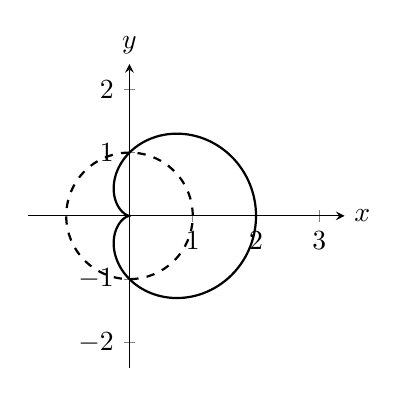
\begin{tikzpicture}
\begin{axis}[width=5.6cm,height=5.6cm,axis lines=middle,xmin=-1.6,xmax=3.4,ymin=-2.4,ymax=2.4,xtick={1,2,3},ytick={-2,-1,1,2},axis equal image,xlabel={$x$},ylabel={$y$},
 every axis x label/.style={at={(ticklabel* cs:1)},anchor=west},every axis y label/.style={at={(ticklabel* cs:1)},anchor=south}]
\addplot[thick,domain=0:360,samples=180,data cs=polar]({x},{1+cos(x)});
\addplot[thick,dashed,domain=0:360,samples=90,data cs=polar]({x},{1});
\end{axis}
\end{tikzpicture}
\end{center}
Area inside the cardioid $r=1+\cos\theta$ and outside the circle $r=1$ (dashed): intersections where $\cos\theta=0$, $\theta=\pm\frac\pi2$.
$A=\frac12\int_{-\pi/2}^{\pi/2}\big((1+\cos\theta)^2-1\big)\,d\theta=\frac12\int_{-\pi/2}^{\pi/2}(2\cos\theta+\cos^2\theta)\,d\theta=\frac12\left(4+\frac\pi2\right)=2+\frac\pi4$. \answer{$2+\frac\pi4$.}
\end{example}

\begin{trap}
$\int\cos^2\theta\,d\theta$ needs the identity $\cos^2\theta=\frac{1+\cos2\theta}{2}$. And the polar area formula has a $\frac12$; leaving it out doubles the answer.
\end{trap}

\section{Common errors}
\begin{itemize}
\item $\frac{d^2y}{dx^2}=\frac{y''(t)}{x''(t)}$ (R9.2).
\item Giving speed as a vector, or velocity as a number (R9.4).
\item Position without the initial value (R9.5).
\item Deciding ``toward the origin'' from $\frac{dr}{d\theta}$ alone when $r<0$ (R9.8).
\item Missing the $\frac12$, or $\frac12\int(r_1-r_2)^2$ in polar area (R9.9--R9.10).
\end{itemize}

\end{document}
